
\documentclass[12pt, addpoints]{exam}
\usepackage[utf8]{inputenc}
\usepackage[portuguese]{babel}
\usepackage{multicol}
\usepackage{graphicx}
\usepackage{amsmath}
\usepackage{xcolor}
\usepackage[a4paper, portrait, margin=2cm]{geometry}

\setlength{\columnsep}{1cm}

\begin{document}

        
\begin{minipage}[l]{0.5\linewidth}
    \begin{flushleft}
        {\bf \Large Prova bimestral}
    \end{flushleft}
\end{minipage}
\begin{minipage}[r]{0.45\linewidth}
    \begin{flushright}
        {\bf \Large Código: XXXXX}
    \end{flushright}
\end{minipage}
\vspace{0.5cm} \hrule \vspace{0.5cm}
\begin{minipage}{0.75\linewidth}
    Aluno:
\end{minipage}
\begin{minipage}{0.20\linewidth}
    Data: 
\end{minipage}
\vspace{0.5cm} \hrule \vspace{0.5cm}
\begin{center}
    \textcolor{red}{\large Versão de correção}
\end{center}

\begin{questions}
\begin{multicols}{2}
\question[33] Durante sua trajetória uma partícula realizou um trabalho de   -2.66 J. Qual foi a variação da sua energia cinética?

\begin{oneparchoices}
\choice -3.57 J\choice 3.4 J\choice -0.09 J\choice -9.7 J\choice -7.86 J\choice -6.99 J\choice -2.66 J\choice 3.3 J\choice -0.28 J\choice 6.47 J\end{oneparchoices}

\begin{oneparchoices}
\choice 0.0\choice 0.0\choice 0.0\choice 0.0\choice 0.0\choice 0.0\choice 33\choice 0.0\choice 0.0\choice 0.0\end{oneparchoices}
\question[23] Considere uma partícula de massa    3.34 kg e velocidade    1.92 m/s. Determine a sua energia cinética.

\begin{center}
\begin{minipage}[c]{0.75\linewidth}
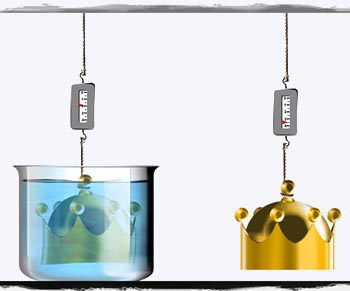
\includegraphics[width=\textwidth]{MWE001.jpg}
\end{minipage}

\end{center}
\begin{oneparchoices}
\choice 3.99 J\choice 176.87 J\choice 429.29 J\choice 8.75 J\choice 10.57 J\choice 9.48 J\choice 203.61 J\choice 71.7 J\choice 113.4 J\choice 6.15 J\end{oneparchoices}

\begin{oneparchoices}
\choice 0.0\choice 0.0\choice 0.0\choice 0.0\choice 0.0\choice 0.0\choice 0.0\choice 0.0\choice 0.0\choice 23\end{oneparchoices}
\end{multicols}
\end{questions}
\newpage
\begin{minipage}[l]{0.5\linewidth}
    \begin{flushleft}
        {\bf \Large Prova bimestral}
    \end{flushleft}
\end{minipage}
\begin{minipage}[r]{0.45\linewidth}
    \begin{flushright}
        {\bf \Large Código: XXXXX}
    \end{flushright}
\end{minipage}
\vspace{0.5cm} \hrule \vspace{0.5cm}
\begin{minipage}{0.75\linewidth}
    Aluno:
\end{minipage}
\begin{minipage}{0.20\linewidth}
    Data: 
\end{minipage}
\vspace{0.5cm} \hrule \vspace{0.5cm}
\begin{center}
    \textcolor{red}{\large Versão de correção}
\end{center}

\begin{questions}
\begin{multicols}{2}
\question[33] Durante sua trajetória uma partícula realizou um trabalho de    2.63 J. Qual foi a variação da sua energia cinética?

\begin{oneparchoices}
\choice -9.96 J\choice 8.47 J\choice 3.24 J\choice 2.63 J\choice 0.52 J\choice 5.55 J\choice 0.47 J\choice 6.22 J\choice -6.47 J\choice 2.18 J\end{oneparchoices}

\begin{oneparchoices}
\choice 0.0\choice 0.0\choice 0.0\choice 33\choice 0.0\choice 0.0\choice 0.0\choice 0.0\choice 0.0\choice 0.0\end{oneparchoices}
\question[23] Considere uma partícula de massa    8.19 kg e velocidade    8.49 m/s. Determine a sua energia cinética.

\begin{center}
\begin{minipage}[c]{0.75\linewidth}
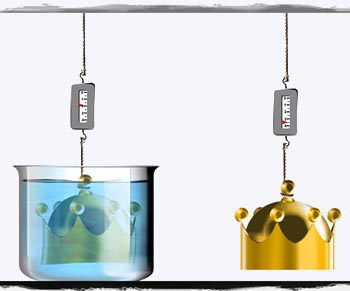
\includegraphics[width=\textwidth]{MWE001.jpg}
\end{minipage}

\end{center}
\begin{oneparchoices}
\choice 486.66 J\choice 44.83 J\choice 609.66 J\choice 21.88 J\choice 38.65 J\choice 34.05 J\choice 294.94 J\choice 511.71 J\choice 6.14 J\choice 22.68 J\end{oneparchoices}

\begin{oneparchoices}
\choice 0.0\choice 0.0\choice 0.0\choice 0.0\choice 0.0\choice 0.0\choice 23\choice 0.0\choice 0.0\choice 0.0\end{oneparchoices}
\end{multicols}
\end{questions}
\newpage
\end{document}
        